\section{Towards Online RLHF for Speech LLM} \label{sec:rlhf}
\begin{figure}[!t]
    \centering
    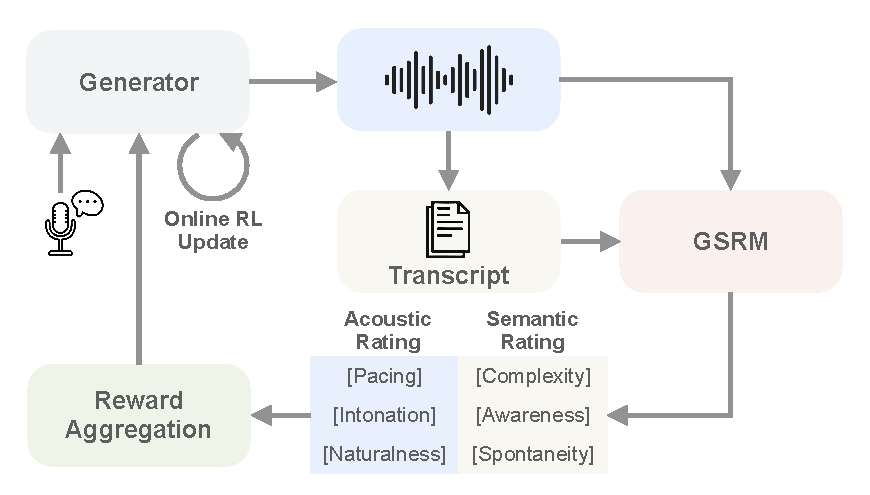
\includegraphics[width=0.7\textwidth]{Figures/rlhf.pdf}
\caption{\textbf{GSRM for Speech Online RLHF.}
Given a user query, a speech LLM acting as the generator produces a spoken response. Both the generated speech and its text transcript are provided to GSRM, which outputs ratings across multiple acoustic and semantic dimensions. A reward aggregator combines these ratings into a scalar reward that is used as feedback to guide online reinforcement learning updates for the generator.}
\label{fig:rlhf}
\vspace{-1em}
\end{figure}
In this section, we study how to leverage GSRM to improve the speech generation quality of a real-time dialogue system, specifically, an in-house speech LLM through online reinforcement learning from human feedback (RLHF).

\textbf{Extending GSRM to Speech Semantic Judgment.} We first note that speech RLHF poses unique challenges compared to text domain. Spoken responses convey rich information along two intertwined dimensions: \emph{acoustic quality}, including intonation and pacing, and \emph{semantic quality}, such as contextual relevance and coherence. To address this, we extend GSRM beyond acoustic evaluation to also judge the semantic quality of speech. Following the same design principles used for naturalness prediction, we define a set of sub-metrics for speech semantic quality, including language complexity, contextual awareness, and spontaneity. We then collect a diverse training set consisting of textual transcripts of real audio responses generated by our in-house speech LLM. These transcripts are annotated by a multi-agent framework, and high-quality CoT reasoning is synthesized using a teacher model. Finally, we fine-tune GSRM on this synthesized dataset to perform semantic judgment. Additional details are provided in Appendix~\ref{sec:semantic_judge}.


\textbf{Applying GSRM to Online RLHF.} Online reinforcement learning has been widely adopted to improve the reasoning capabilities of text LLMs~\cite{zha2025rl,shen2025satori,guo2025deepseek}, yet its potential for improving the generation quality of speech LLMs remains largely unexplored. A key difference lies in the nature of verification: while RL for reasoning tasks often relies on objective signals, RL for speech generation requires \emph{subjective} evaluation across multiple dimensions. GSRM provides a practical solution to this challenge by serving as a universal verifier. As illustrated in Figure~\ref{fig:rlhf}, given a user query, the speech LLM produces spoken responses as rollouts in a real-time interaction loop. Each speech response is transcribed into text using a lightweight automatic speech recognition (ASR) model, such as Whisper~\cite{radford2023robust}, to disentangle semantic content from acoustic characteristics. The generated speech and its corresponding transcript are then provided to GSRM, which predicts ratings across multiple acoustic and semantic dimensions. These ratings are aggregated into a scalar reward according to a predefined aggregation rule. The generator is then iteratively updated by alternating between producing new speech samples and receiving verification feedback from GSRM via an online RL algorithm.
